\documentclass{report}
\usepackage{tikz}
\usepackage[utf8]{vietnam}
\usepackage[english]{babel}
\usepackage{fancyhdr} 
\usepackage{parskip}
\usepackage[left=2cm,right=2cm,top=2cm,bottom=2cm]{geometry}
\usepackage{amsmath,amsxtra,amssymb,latexsym, amscd,amsthm}
\usepackage{algorithm}
\usepackage[noend]{algpseudocode}
\usepackage{listings}
\usepackage{multirow, tabularx}
\usepackage{booktabs}
\usepackage{graphicx}
\usepackage{subfigure}
\usepackage{array}
\usepackage[T5]{fontenc}
\usepackage{colortbl}
\usepackage{listings}
\usepackage{hyperref}

\DeclareFontShape{T5}{cmr}{bx}{sc}{<->ssub * cmr/bx/n}{}
\usetikzlibrary{calc}
\setcounter{secnumdepth}{5} 
\newcommand\tab[1][1cm]{\hspace*{#1}}
\newcommand\HRule{\rule{\textwidth}{1pt}}

\definecolor{codegreen}{rgb}{0,0.6,0}
\definecolor{codegray}{rgb}{0.5,0.5,0.5}
\definecolor{codepurple}{rgb}{0.58,0,0.82}
\definecolor{backcolour}{rgb}{0.95,0.95,0.92}

\lstdefinestyle{mystyle}{
  backgroundcolor=\color{backcolour},   
  commentstyle=\color{codegreen},
  keywordstyle=\color{magenta},
  numberstyle=\tiny\color{codegray},
  stringstyle=\color{codepurple},
  basicstyle=\ttfamily\large,
  breakatwhitespace=false,         
  breaklines=true,                 
  captionpos=b,                    
  keepspaces=true,                 
  numbers=left,                    
  numbersep=7.5pt,                  
  showspaces=false,                
  showstringspaces=false,
  showtabs=false,                  
  tabsize=2,
  % font size is 12pt
  basicstyle=\fontsize{12}{12}\selectfont
}

\lstset{style=mystyle}

\begin{document}

% ========================== TITLE PAGE =============================
\begin{titlepage}

\begin{tikzpicture}[remember picture, overlay]
    \draw[line width = 4pt] ($(current page.north west) + (2cm,-2cm)$) rectangle ($(current page.south east) + (-2cm,1.7cm)$);
\end{tikzpicture}

\begin{center}
% -------------------- Upper part of the page
\textsc{\Large \textbf{VNUHCM - UNIVERSITY OF SCIENCE}}\\

\bigskip

\textsc{\Large FACULTY OF INFORMATION TECHNOLOGY}\\

\bigskip

% -------------------- University Logo
\begin{figure}[!h]
    \centering
    \includegraphics[width=5.2cm, height=5.2cm]{logo.png}
\end{figure}

% -------------------- Title
\HRule \\[0.4cm]
{\huge\bfseries \textcolor{blue}{LAB 03 REPORT}}\\[0.4cm]
{\Large\bfseries COMPUTER VISION}
\HRule \\[1cm]

% -------------------- Student name
\begin{center}
    \textbf{\Large Lâm Thanh Ngọc - 21127118} \\
    \medskip
    \Large{\textbf{Class: 21TGMT}}\\[4cm]
\end{center}

% -------------------- Advisor name
\begin{center}
    \textbf{\Large Lecturers: \\[0.2cm]}
    \Large{Phạm Minh Hoàng \\[0.2cm] Nguyễn Trọng Việt \\ [0.2cm] Võ Hoài Việt}
\end{center}
\vfill

% ------------------------ Bottom of the page

{\today}
\end{center}
\end{titlepage}
% ===================== END OF TITLE PAGE ==========================



% ======================== HEADER AND FOOTER ======================
\pagestyle{fancy}
\setlength{\headheight}{0.5cm}
\fancyhf{}
\lhead{\textbf{LAB 03}}
\rhead{\textbf{Computer Vision}}
\rfoot{Page \thepage}
% ==================== END OF HEADER AND FOOTER =====================



% ====================== TABLE OF CONTENTS ==========================
\Large
\tableofcontents
\thispagestyle{fancy} % Fix footer and header
\vfill
\pagebreak
% ===================== END OF TABLE OF CONTENTS ==================



% =============== SECTION AND SUBSECTION NUMBERING ==================
\renewcommand\thesection{\arabic{section}} % Section start from 1,2,3...
\renewcommand\thesubsection{\thesection.\arabic{subsection}} % Subsection start from 1,2,3,...
\renewcommand\thesubsubsection{\alph{subsection}} 
% ============ END OF SECTION AND SUBSECTION NUMBERING ==============

%============= CONTENT =============
\section{Evaluation}

\begin{table}[h!]
\centering
\begin{tabular}{lllll}
\cline{1-3}
\multicolumn{1}{|c|}{\cellcolor[HTML]{010066}{\color[HTML]{FFFFFF} \textbf{Manipulation}}} &
  \multicolumn{1}{c|}{\cellcolor[HTML]{010066}{\color[HTML]{FFFFFF} \textbf{Level of completion}}} &
  \multicolumn{1}{c|}{\cellcolor[HTML]{010066}{\color[HTML]{FFFFFF} \textbf{Evaluation}}} &
   \\ \cline{1-3}
\multicolumn{1}{|l|}{Object detection using Local Feature} &
  \multicolumn{1}{l|}{100\%} &
  \multicolumn{1}{l|}{Completed} &
   \\ \cline{1-3}
\end{tabular}
\centering
\end{table}
%==========================================
\section{Users guide}
\begin{itemize}
  \item[2.1.] Open the terminal and navigate to the folder containing the source code.
  \item[2.2.] Run the command \textcolor{blue}{\lstinline|21127118.exe|} to execute the program.
  \item[2.3.] Then, the program will show the valid command: \\ \textcolor{blue}{\lstinline|<Executable file> -sift <TemplateImagePath> <SceneImagePath> <OutputFilePath>|}
  \begin{itemize}
    \item[-] \textcolor{blue}{\lstinline|<Executable file>|} is 21127118.exe.
    \item[-] \textcolor{blue}{\lstinline|TemplateImagePath|} and \textcolor{blue}{\lstinline|SceneImagePath|} are the paths to the template and scene images.
    \item[-] \textcolor{blue}{\lstinline|OutputFilePath|} is the path to the output image.
  \end{itemize}
  \item[2.4.] For example: \\ \textcolor{blue}{21127118.exe -sift Input$\setminus$temp.jpg Input$\setminus$scene.jpg Output$\setminus$Result.jpg}
\end{itemize}

%===========================================

\section{Function description}
In the code, there are 3 supporting functions: 

\begin{itemize}
  \item[-] \textcolor{blue}{\lstinline|Mat read_image(string path)|} is used to read the image from the given path with the \textcolor{blue}{\lstinline|imread(path, IMREAD_COLOR)|} function of OpenCV.
  \item[-] \textcolor{blue}{\lstinline|void show_and_save(string name, Mat image, string save_path)|} is used to show the image and save it to the given path with the \textcolor{blue}{\lstinline|imshow()|} and \textcolor{blue}{\lstinline|imwrite()|} functions of OpenCV.
  \item[-] \textcolor{blue}{\lstinline|void draw_bb(Mat& scene, Mat& temp, Mat H)|} is used to draw the bounding box around the object in the scene image with the \textcolor{blue}{\lstinline|perspectiveTransform()|} function of OpenCV.
\end{itemize}

\subsection*{SIFT algorithm}
The SIFT algorithm is used widely in computer vision for object recognition, image stitching, and 3D reconstruction.

The algorithm follows these steps:
\begin{itemize}
  \item[1.] Scale-space peak selection: Keypoints (or interest points) in an image are detected using the difference of Gaussian (DoG) function to identify locations where the DoG is maximized.
  \item[2.] Keypoint Localization: Detected keypoints are localized to reduce unnescary points by using Taylor series expansion and checking the intensity at the detected point. If the intensity is less than a threshold, the point is discarded.
  \item[3.]Orientation Assignment: For the purpose of stability, the orientation of the keypoint is assigned by creating a histogram of the gradient directions of the pixels in a region around the keypoint. The highest peak in the histogram is considered as the orientation of the keypoint.
  \item[4.] Keypoint Descriptior: A descriptor is computed by creating a 16x16 grid around the keypoint which is divided into 16 sub-blocks of 4x4 pixels. The gradient magnitude and orientation of each pixel in the sub-block are used to create a 128-dimensional vector.
  \item[5.] Keypoint Matching: Once descriptors are computed for all keypoints in the image, the nearest neighbor algorithm is used to match the keypoints between the template and the scene image.
\end{itemize}

The algorithm is implemented with the following functions:

\textbf{\textcolor{blue}{\lstinline|void detect_and_compute(Mat img, vector<KeyPoint>& kps, Mat& desc)|}}

\textbf{Description:} The function is used to detect keypoints and compute the descriptors for the given image.

\textbf{Implementation:} From the initialized SIFT Ptr<Feature2D> object by \textcolor{blue}{\lstinline|SIFT::create()|}, the function \textcolor{blue}{\lstinline|detectAndCompute()|} is used to detect keypoints and compute the descriptors for the given image with Mat() as the mask.

\textbf{\textcolor{blue}{\lstinline|vector<DMatch> match_descriptors(Mat descriptors1, Mat descriptors2)|}}   

\textbf{Description:} The function is used to match the descriptors between the template and the scene image using the FLANNBASED matcher and the KNN match.

\textbf{Implementation:} After initializing the FLANNBASED object with \textcolor{blue}{\lstinline|DescriptorMatcher::create(DescriptorMatcher::FLANNBASED)|}, the function \textcolor{blue}{\lstinline|knnMatch()|} is called in order to match the descriptors between the template and the scene image.

The return value is a DMatch vector which contains the index of the best match for each descriptor in the template and the scene image calculated with the condition that the distance of the best match is less than 0.75 times the distance of the second best match.

\pagebreak
\textbf{\textcolor{blue}{\lstinline|Mat Homography(vector<KeyPoint> keypoints1, vector<KeyPoint> keypoints2, vector<DMatch> good_matches)|}}

\textbf{Description:} The function is used to find the homography matrix between the template and the scene image using the RANSAC algorithm.

\textbf{Implementation:} The 2 vectors of keypoints are initialized by getting the coordination of query index and train index from the good matches among the 2 vectors of keypoints in the template and the scene image.

The function then uses \textcolor{blue}{\lstinline|findHomography()|} is used to find the homography matrix between the 2 keypoints vector with the RANSAC algorithm and the RANSAC threshold is set to 3.

\section{Proof images}
\begin{figure}[h!]
  \centering
  \subfigure[Template image]{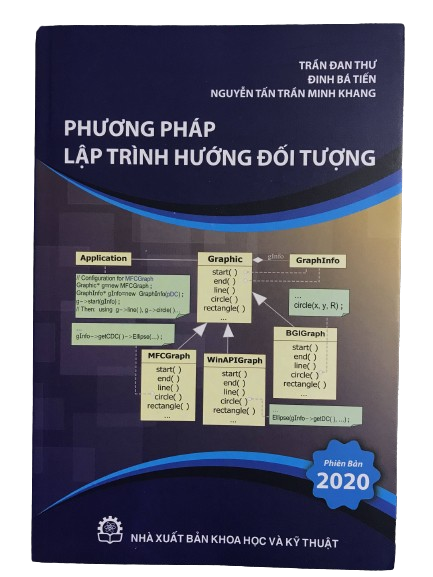
\includegraphics[width=0.4\textwidth]{temp.png}}
  \subfigure[Scene image]{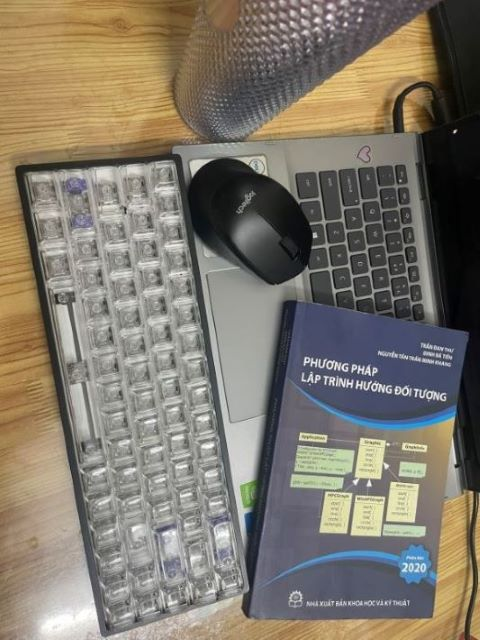
\includegraphics[width=0.4\textwidth]{scene.jpg}}
  \caption{Template and Scene images}
\end{figure}

\begin{figure}[h!]
  \centering
  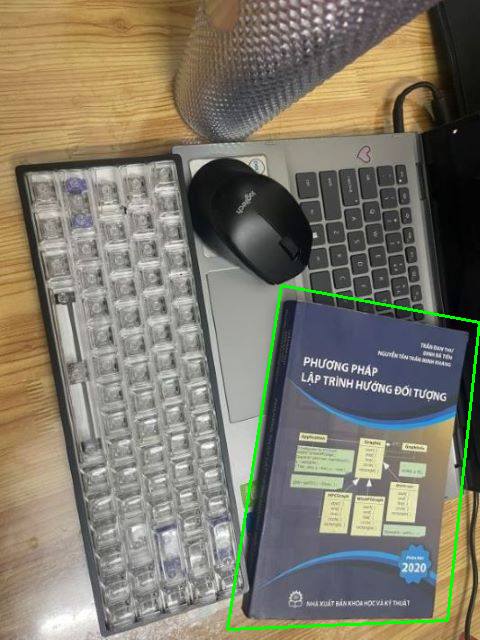
\includegraphics[width=0.6\textwidth]{result.png}
  \caption{Result image}
\end{figure}

\pagebreak
\section{References}
\begin{itemize}
  \item[] Lab02 document on moodle.
  \item[] \href{https://medium.com/@deepanshut041/introduction-to-sift-scale-invariant-feature-transform-65d7f3a72d40}{SIFT algorithm.}
  \item[] \href{https://github.com/tdkhan/object-detection-SIFT}{Object detection using SIFT.}
\end{itemize}

\end{document}